\chapter{Data}
\label{cha:data}

This chapter describes the spatio-temporal dataset used in the thesis project.
The dataset provider is briefly mentioned alongside the data gathering process, followed by the structure of the data.
The structure of the data describes the different event types in the dataset and how they were used in the thesis project.
After the basic characteristics of the dataset has been described the pre-processing steps applied are described and motivated.
The pre-processing section also covers problems inherent in the dataset and the solutions employed to remedy them.
The problems are visualised by real-world examples.

\section{Background}
The dataset was provided by Östgötatrafiken AB and contains \todo{300?}GB of data.
Östgötatrafiken AB is owned by Östergötland County and is responsible for the public transportation in the county.
This thesis project only analysed the bus data available in the given data set.
The dataset is a collection of documents, where one document represents a full day of data.
A typical day has a document size of around \todo{2.5?}GB.

\subsection{Data Gathering}
The process of gathering the data used in this thesis project can be generally described by the following simplified procedure:
\begin{enumerate}
    \item Each Östgötatrafiken AB bus is running a system collecting data from sensors installed inside the bus.
    \item The system collects the sensor data and transmits it to a central server or database.
    \item A log containing all events for a full day is created and stored as a document in a collection.
    \item The central server processes and analyses the data. The results from the data analysis is stored in the log.
\end{enumerate}

\begin{figure}
    \centering
    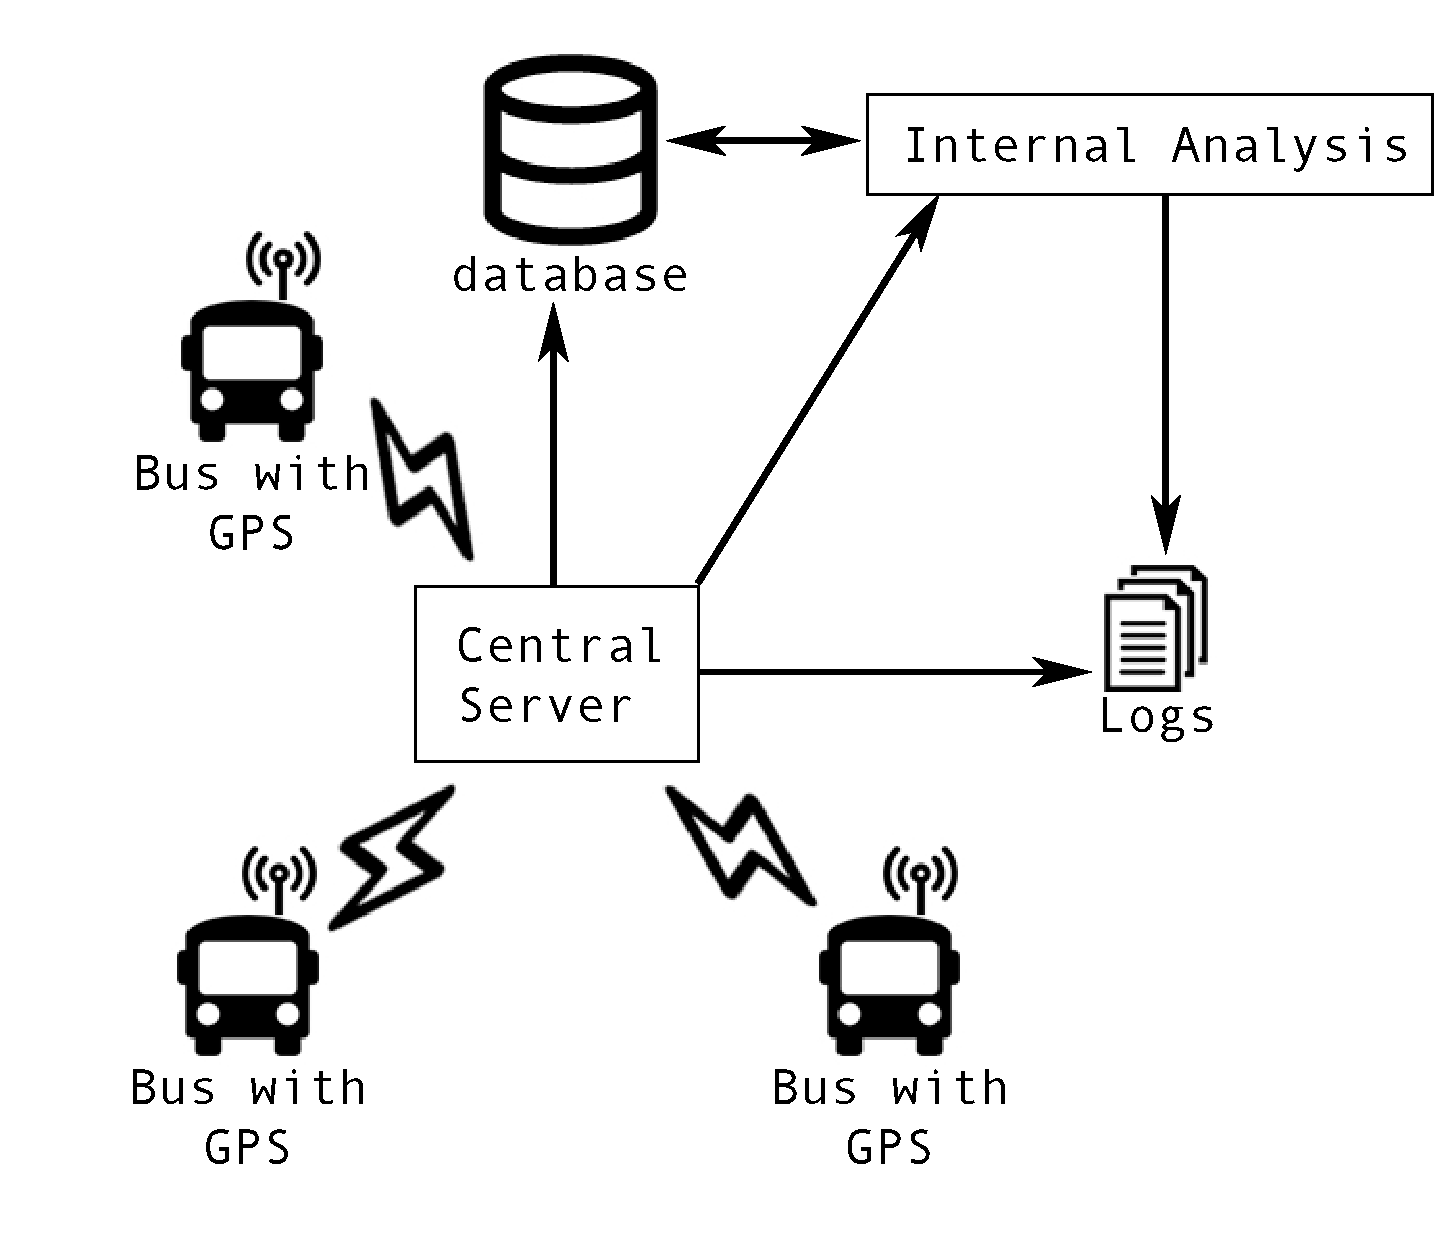
\includegraphics[width=0.75\textwidth]{figures/data-gathering}
    \caption{Simplified graph illustrating the data gathering process. Each bus is equipped with a GPS sensor and transmits its position to a central server/database.
    The dataset used in this thesis project is the log, which is a collection of documents.
    Each document contains the GPS data sent from all buses during a single day, together with data from the "Internal Analysis" component of the server.}
    \label{fig:data-gathering}
\end{figure}

Figure \ref{fig:data-gathering} illustrates the procedure.
The collection of logs is the dataset used in this thesis project.
The logs contain the GPS data from the buses and also events created by the "Internal Analysis" component in the system.
The precise implementation of the "Internal Analysis" component is unknown.

\section{Structure} \label{sec:data-structure}
A document in the dataset is made up of a large number of events representing a single day.
A single day typically contains roughly 21 \todo{Is it interesting to plot this exact number and its variance?} million events.  
Each event is represented by a single line of text.
An event can be split into two groups: a header and a body.
There are different types of events reported during the span of a single day.
Each type has its own header and body structure.

\subsection{Event Example}

\begin{figure}[ht!]
    \centering
    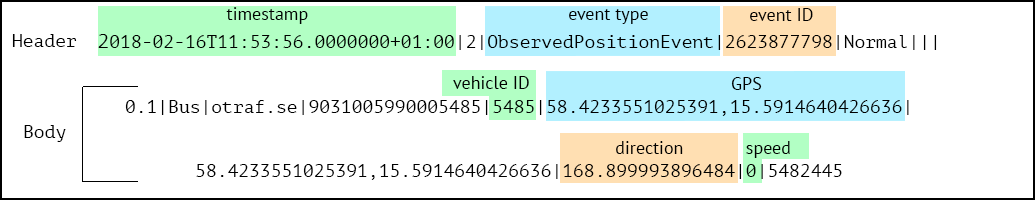
\includegraphics[width=\textwidth]{figures/data-example-1}
    \caption{Example of a raw \texttt{ObservedPositionEvent} entry.
    The header and the body is separated by \texttt{|||}.
    Each parameter in the header and body is separated by a single \texttt{|}.
    Key parameters for the \texttt{ObservedPositionEvent} event type is highlighted.}
    \label{fig:data-ex-1}
\end{figure}

Figure \ref{fig:data-ex-1} illustrates an event with the event type \texttt{ObservedPositionEvent}.
The header is defined as all the parameters before the \texttt{|||} separator.
All the parameters after the separator is defined as the body of the event.
In this example the header and body contain seven key parameters: 
\begin{itemize}
    \item \textit{Timestamp:} A timestamp (\texttt{2018-02-16T11:53:56.0000000+01:00}), which is the timestamp from the system running on the bus.
    \item \textit{Event Type:} The event type (\texttt{ObservedPositionEvent}).
    \item \textit{Event ID:} The event id (\texttt{2623877798}). This is a number set by the system responsible for collecting the data from all buses.
    It is incremented for every event added to the log by either the database system or the "Internal Analysis" component in Figure \ref{fig:data-gathering}.
    \item \textit{Vehicle ID:} Unique ID for the bus transmitting its position.
    \item \textit{GPS:} The GPS position of the bus in latitude and longitude.
    \item \textit{Direction:} The direction of the bus.
    \item \textit{Speed:} The current speed of the bus.
\end{itemize}

\subsection{Event Types}
The dataset contains 20 unique event types.
Figure \ref{fig:types-barplot} visualises the distribution of event types for an arbitrary day \todo{Should we instead do a boxplot of the whole dataset? Will take a lot of time to create!} in the dataset.
The figure only gives an indication of what the true distribution could be, as it is computationally expensive to calculate the true distribution for the given dataset, due to its size.
Knowledge about the true distribution is not required in order to reason about the event types.
As the figure shows, the majority of events that occur are of the type \texttt{ObservedPositionEvent}, which is the event containing an updated GPS position for a vehicle.

\begin{figure}[ht!]
    \centering
    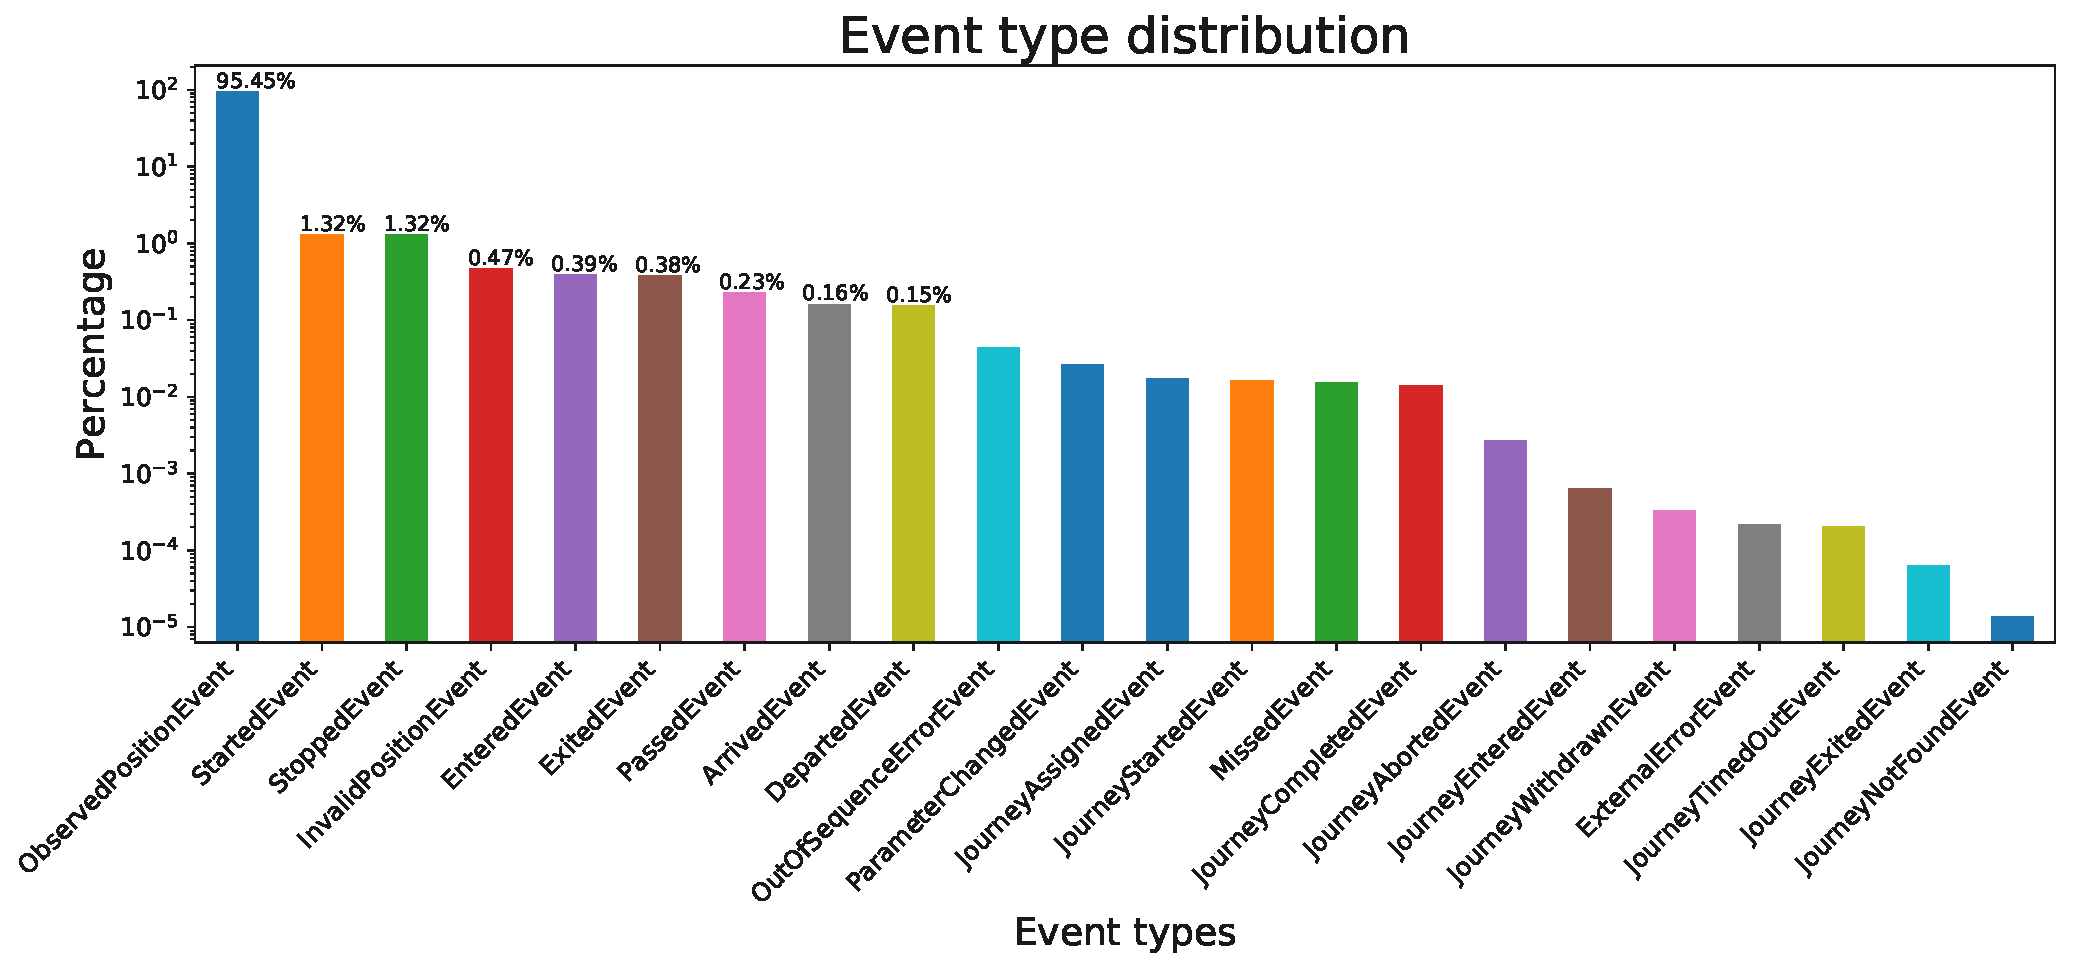
\includegraphics[width=\textwidth]{figures/types_barplot}
    \caption{The distribution of event types for a random day in the dataset.}
    \label{fig:types-barplot}
\end{figure}

Of the 20 event types available in the dataset, this thesis project only used 12 of them.
The events to use were chosen by analysing the log for a single day in great detail.
Event types which occurred rarely and seemingly random were discarded, as no pattern could be determined for them.
The \texttt{InvalidPositionEvent} type only contains the GPS position of the vehicle.
The valid \texttt{ObservedPositionEvent} type also contains the \textit{Speed} and \textit{Direction} parameters.
The GPS position of the \texttt{InvalidPositionEvent} events were always the same coordinates.
In this thesis project the \texttt{InvalidPositionEvent} type was discarded, due to the missing parameters and static GPS position.

The 12 event types used in this thesis project were:
\begin{itemize}
    \item \textit{ObservedPositionEvent}:
    This event type contains the information highlighted in Figure \ref{fig:data-ex-1}.
    It is the most prevalent event type in the provided dataset.
    This event type is contextless, as it contains no information about which public transportation line the vehicle is currently serving, if any. 
    
    \item \textit{StartedEvent} and \textit{StoppedEvent}:
    These two event types provide context to a sequence of observed position events.
    They denote when the vehicle has started or stopped moving, respectively.
    For example, they can be used to identify road intersections, bus stops, traffic or driver breaks.
    
    \item \textit{EnteredEvent} and \textit{ExitedEvent}:
    These two event types are used by the "Internal Analysis" component to identify bus stops.
    The \textit{EnteredEvent} is produced by the system when the vehicle is within a certain predefined distance to a bus stop.
    The \textit{ExitedEvent} is similarly produced when the vehicle leaves the predefined distance to the bus stop.
    These event types could, for example, be used in an algorithm which improves the bus stop detection.
    
    \item \textit{PassedEvent}, \textit{ArrivedEvent}, and \textit{DepartedEvent}:
    These three event types are used to provide information regarding which bus stop a particular bus is at.
    The \textit{PassedEvent} type denotes when a particular bus, serving a specific public transportation line, passed a bus line stop.
    It contains information about the predefined position of the stop, the public transportation line the particular bus is currently serving and the time of the passing.
    Similarly, the \textit{ArrivedEvent} and \textit{DepartedEvent} types denote when a particular bus arrived at or departed from a particular bus stop.
    These event types provide context to the observed positions.
    In this thesis project they are used to group a sequence of observed positions into a segment between two stops for a particular bus line.
    
    \item \textit{ParameterChangedEvent}:  
    The \textit{ParameterChangedEvent} type is the most dynamic event type in the data set, e.g. it can be used to inform the system when the doors on a particular bus open or close or when a bus changes journeys.
    In this thesis project it is only used to identify bus lines and give context to observed positions.
    
    \item \textit{JourneyStartedEvent} and \textit{JourneyCompletedEvent}:
    The \textit{JourneyStartedEvent} type is produced by the "Internal Analysis" component when a bus has reached the starting bus stop for a bus line.
    The \textit{JourneyCompletedEvent} event type is produced when the bus has reached the final bus stop for a bus line.

    \item \textit{JourneyAssignedEvent}:
    This event type is accompanied by a \textit{ParameterChangedEvent} to denote when a bus changes its journey.
\end{itemize}

\section{Pre-processing Events}
The first step deemed necessary in order to use the data in the provided dataset was to transform it from strings to object with attributes.
Figure \ref{fig:data-ex-1} visualises which attributes an \textit{ObservedPositionEvent} object contains.
Similar structures were created for each of the mentioned event types.

During this pre-process step all the events from a vehicle type other than "Bus" were ignored.
A \textit{geo-fence} was applied in order to facilitate and support manual inspection and visualisation of the data in the dataset.
A geo-fence is a virtual polygon which establishes a virtual perimeter for a real-world geographical area.
The geo-fence applied in this thesis project is shown in Figure \ref{fig:geo-fence}.

\begin{figure}[ht!]
    \centering
    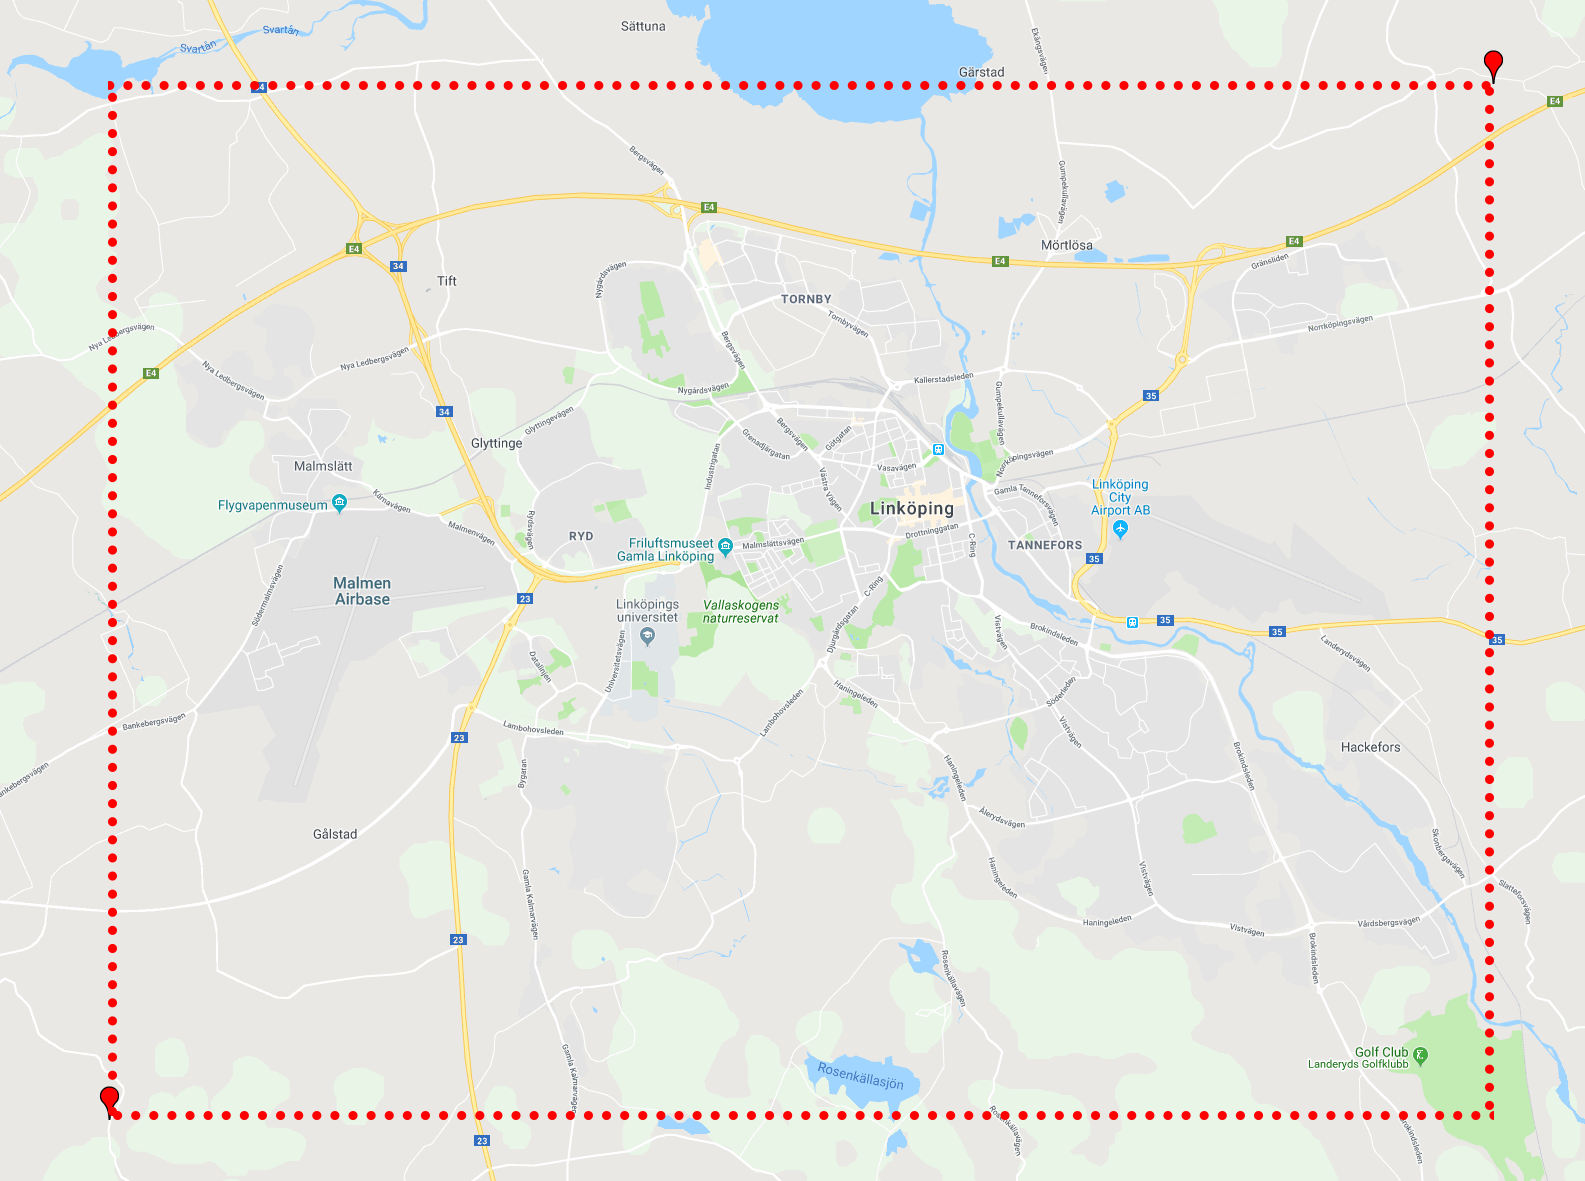
\includegraphics[width=0.9\textwidth]{figures/geofencing_linkoping}
    \caption{A geo-fence is constructed to filter out events occurring outside the virtual perimeter.
    The two red markers create a rectangular boundary, which is illustrated with the red-dotted line.
    The geographical area is the city of Linköping.}
    \label{fig:geo-fence}
\end{figure}

\begin{figure}[ht!]
    \centering
    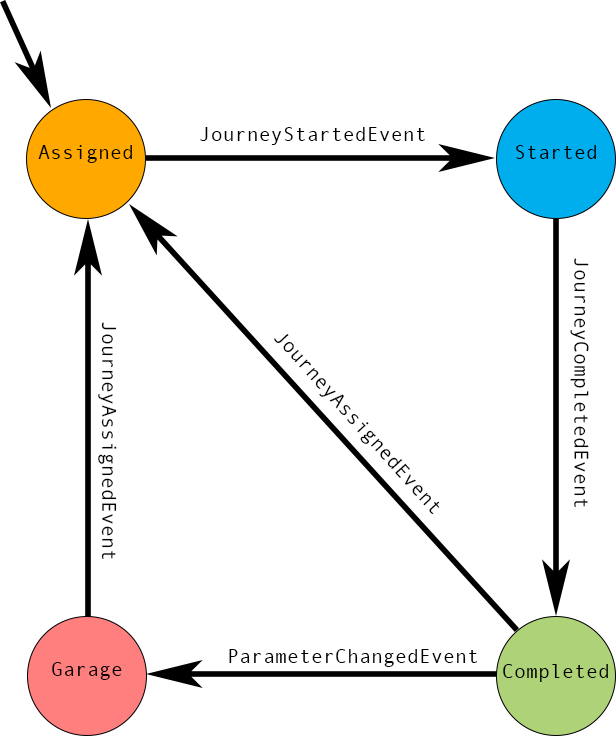
\includegraphics[width=0.7\textwidth]{figures/context-state-machine}
    \caption{Finite-state machine providing context to \textit{ObservedPositionEvent}s. 
    The constructed finite-state machine is simplified to illustrate the best-case scenario.
    The "Assigned" state is the starting state.
    \textit{ObservedPositionEvent}s are assigned to the current state the state machine is in.
    }
    \label{fig:context-state-machine}
\end{figure}

After the parsing and filtering step the idea was to provide context to \textit{ObservedPositionEvent}s.
Only using this one contextless event type greatly reduces the span of potential problems one could solve with the provided dataset.
Context was provided by constructing a finite-state machine.

\subsection{Context-Providing Finite-State Machine}
Finite-state machines are well-defined \todo{what is the formal definition?} and can be modelled with simple algorithmic structures \todo{source?}.
The context-providing finite-state machine constructed in this thesis project is shown in Figure \ref{fig:context-state-machine}.
The shown state machine is illustrating the best-case scenario, when the actual order of events is equal to the logical ordering of events, see Figure \ref{fig:assigned-before-completed-working} for a real-world example.
However, this is not always the case when working with real world data, as shown in Figures \ref{fig:assigned-before-completed-long} and \ref{fig:assigned-before-completed}.
Occasionally the timing of events gets mixed up, e.g. a bus in the "Started" state receives a \textit{JourneyAssignedEvent} before it receives a \textit{JourneyCompletedEvent}.
This ordering breaks the logical ordering of events: a journey needs to be completed before a new one can assigned.

\begin{figure}[h!]
    \centering
    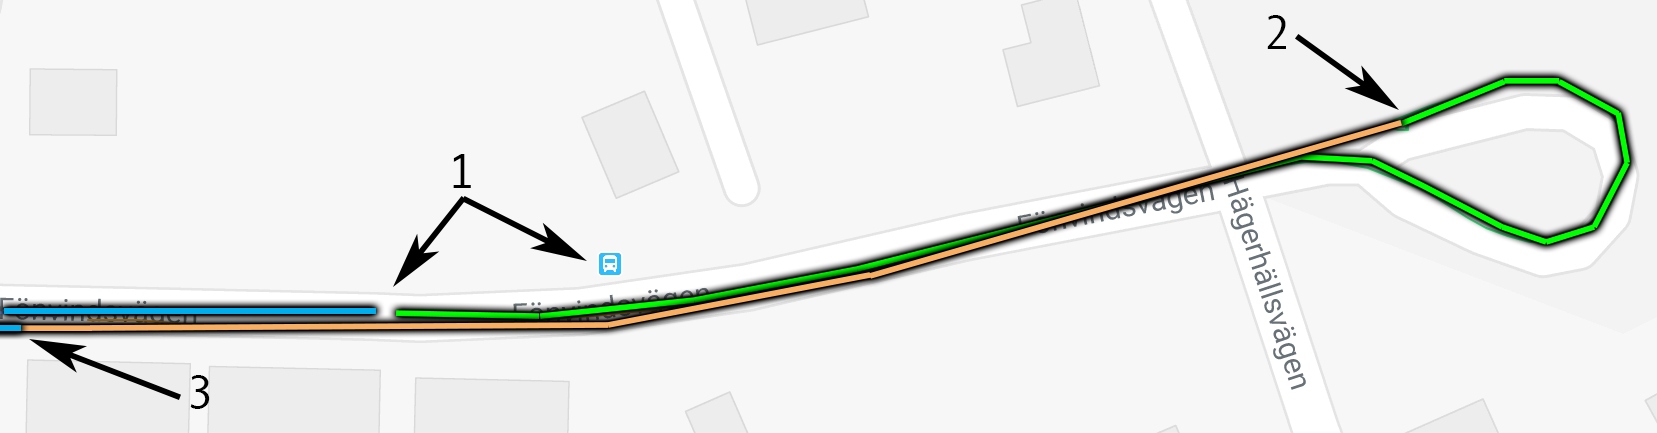
\includegraphics[width=1\textwidth]{figures/assigned_completed_working}
    \caption{Real-world scenario illustrating when events occur in a correct, logical ordering.
    The blue line to the left is \textit{ObservedPositionEvent}s in the "Started" state.
    Upon reaching the final bus stop for the line the state changes to "Completed".
    The \textit{ObservedPositionEvent}s for this state is drawn with a green line to denote the "Completed" state.
    The bus turns around and stops for a period of time until a new bus line is assigned to it.
    In this particular scenario, the bus is assigned the same bus line number, but in the opposite direction.
    The orange line denotes the \textit{ObservedPositionEvent}s in the "Assigned" state.
    Shortly after passing the first bus stop the orange line changes to blue (not shown in the image), which denotes the "Started" state.}
    \label{fig:assigned-before-completed-working}
\end{figure}

\begin{figure}[t!]
    \centering
    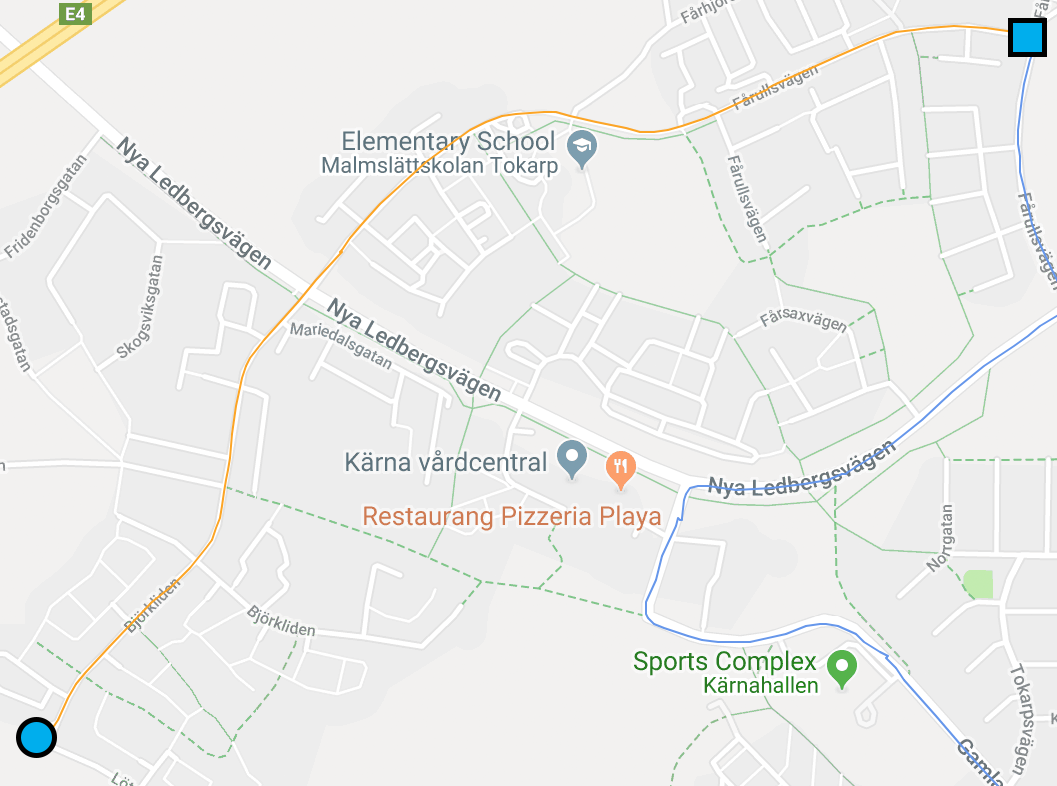
\includegraphics[width=0.75\textwidth]{figures/assigned_completed_problem_long}
    \caption{Example illustrating when the real ordering of events breaks the logical ordering.
    The bus is assigned a new bus line long before reaching the final bus stop.
    The final bus stop is marked with a circle.
    The rectangle marks the position of the bus when it is assigned a new bus line.
    The last part of the journey (the path between the rectangle and the circle) is thus assigned to a new state "Assigned", instead of the actual, logical state "Started".}
    \label{fig:assigned-before-completed-long}
\end{figure}

\begin{figure}[t!]
    \centering
    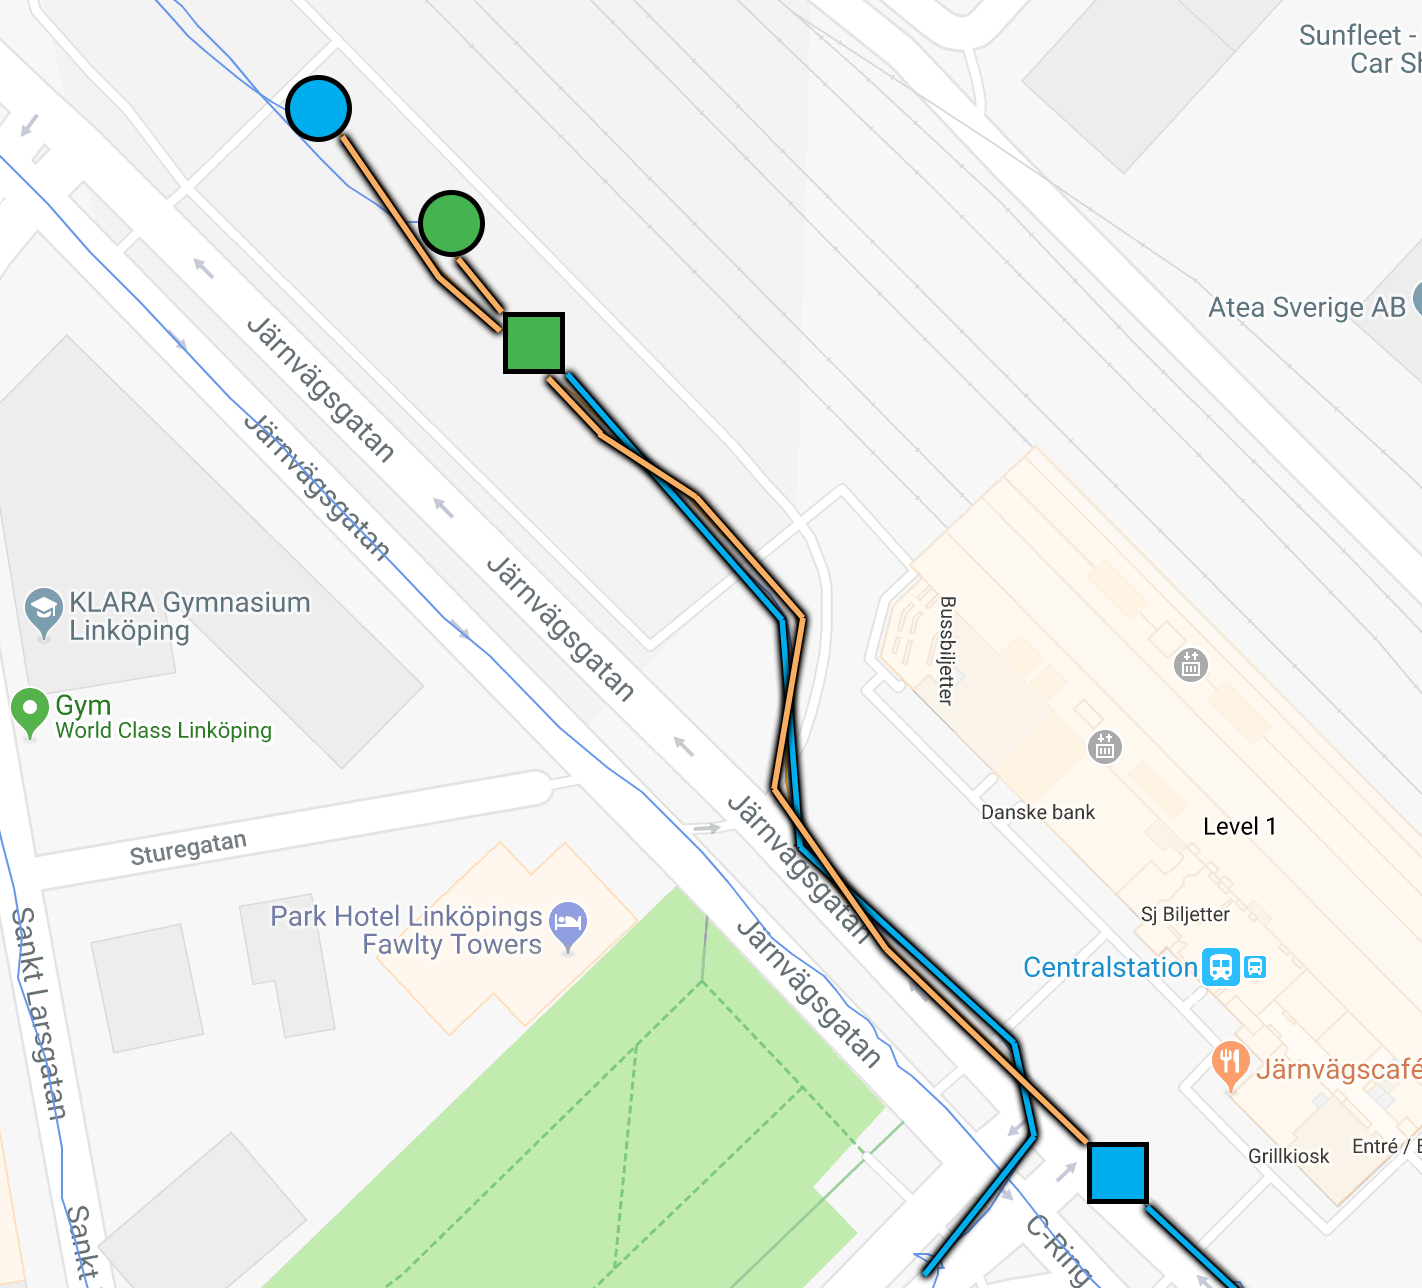
\includegraphics[width=0.75\textwidth]{figures/assigned_completed_problem}
    \caption{Another example illustrating two cases where a bus is assigned a new bus line before completing the started one.
    The two circles (green and blue) denote the final bus stops for the respective bus lines.
    One of the buses is assigned a new bus line at the blue rectangle in the bottom-right corner, long before reaching the final bus stop.
    The other bus is assigned a new bus line at the green rectangle, which is closer to the final bus stops.
    This example demonstrates that the assignment to a new bus line is independent of the distance to the final bus stop.}
    \label{fig:assigned-before-completed}
\end{figure}

The problem is solved by partly changing the ordering of events from \textit{Timestamp} to \textit{Event ID}.
This is a feasible approach when the data is batched into separate files, where one file is a full day of events.
When processing data in real time the approach would have to be slightly altered.
The \textit{ObservedPositionEvent}s would have to be placed in a temporary buffer once an anomaly is detected in the event ordering, e.g. \textit{JourneyAssignedEvent} is received before \textit{JourneyCompletedEvent} and the system is in the "Started" state.
Once the \textit{JourneyCompletedEvent} type is finally received, the data in the buffer could be retroactively added to the "Started" state.
The "Started" state would then correctly contain all \textit{ObservedPositionEvent}s received from the starting bus stop to the final bus stop.

\begin{figure}[t!]
    \centering
    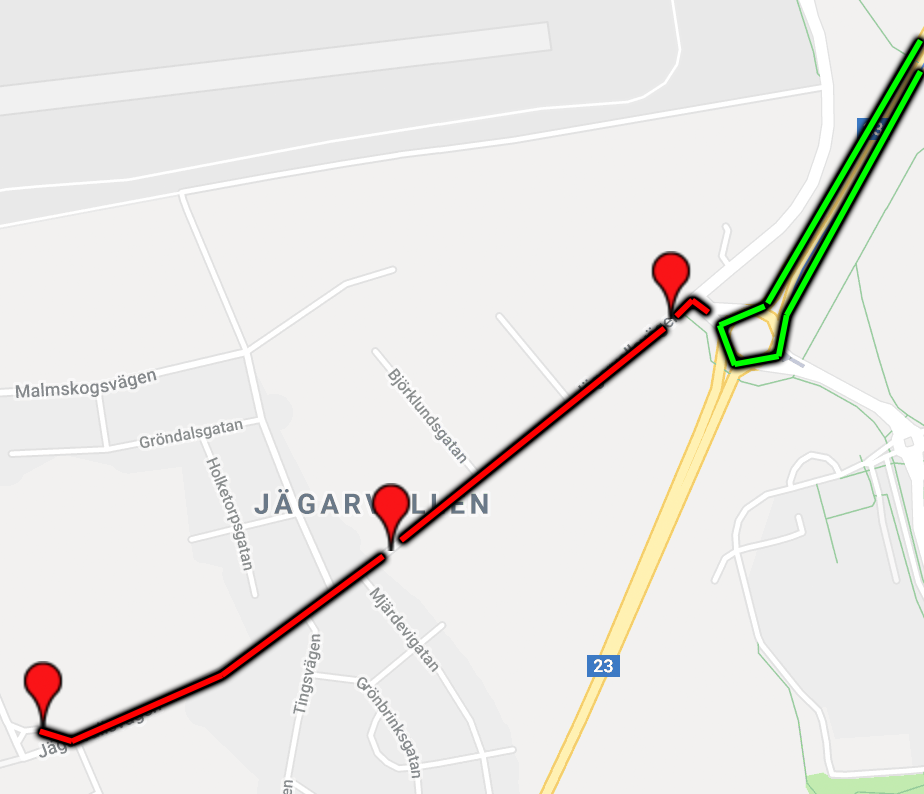
\includegraphics[width=0.6\textwidth]{figures/edge_case_early_quit}
    \caption{Example of early stopping in a journey.
    The three markers are the final three stops of a particular bus line.
    Instead of following the pre-determined route of the bus line, the final three stops are skipped.
    This results in the journey never being deemed completed.}
    \label{fig:human-error-early-stopping-1}
\end{figure}

\begin{figure}[t!]
    \centering
    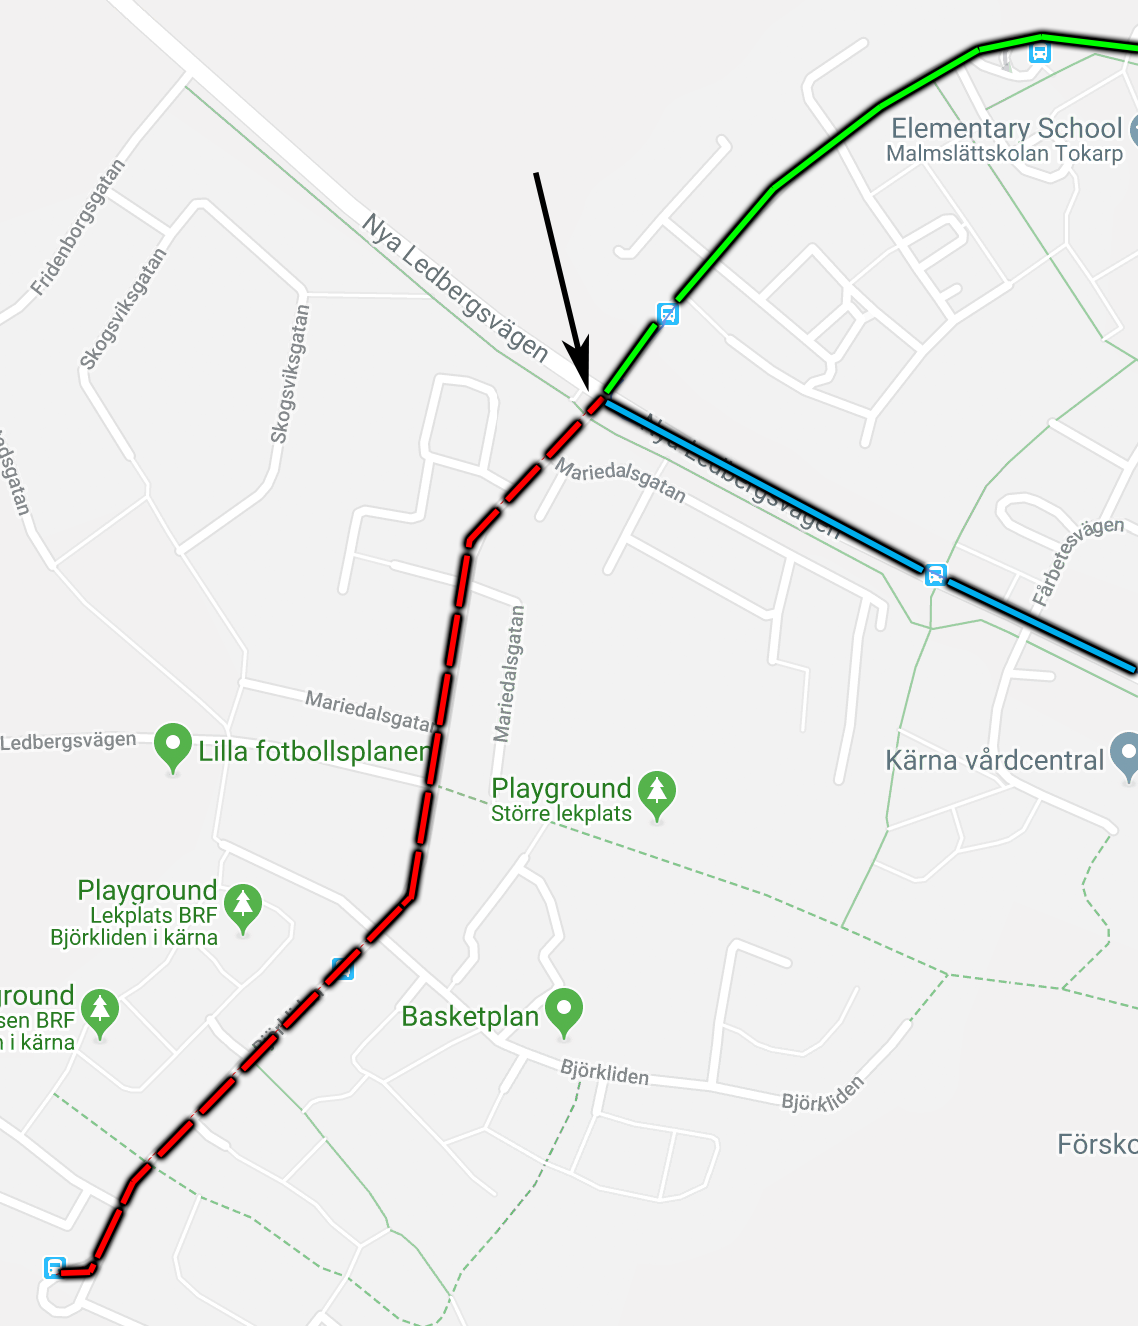
\includegraphics[width=0.65\textwidth]{figures/lazy_driver_2}
    \caption{Another example of early stopping in a journey.
    The red dashed line is the planned route of the bus line.
    The blue line at "Nya Ledbergsvägen" is the actual route the bus drove.
    This results in the journey never being deemed completed, creating a erroneous ordering of contextual events.}
    \label{fig:human-error-early-stopping-2}
\end{figure}

Unfortunately, it is not always the case that the \textit{JourneyCompletedEvent} type is in an erroneous ordering.
Occasionally the type is missing from the sequence of events due to either human errors or imprecise algorithms in the "Internal Analysis" component.

\subsection{Human Error: Early Stopping}
Figure \ref{fig:human-error-early-stopping-1} and \ref{fig:human-error-early-stopping-2} illustrate two scenarios when the \textit{JourneyCompletedEvent} type for a started journey would be missing.
In Figure \ref{fig:human-error-early-stopping-1}, the bus driver is supposed to visit the three markers in order to complete the journey for a particular line.
In Figure \ref{fig:human-error-early-stopping-2}, the dashed line highlights the route of the bus line, while the blue line is the actual route the bus drove.
In both these real-world examples, the bus drivers ignore the final stops of the journeys.

The "Internal Analysis" component never deems the journey as completed in these scenarios, which results in the \textit{JourneyCompletedEvent} type never being produced.
This scenario is easy to detect in historical data, but in real-time certain assumptions need to be made.
For example, if the journey is compared with an average journey, the anomaly could be detected early.
However, it would be uncertain if the anomaly is due to a journey being stopped early or if the bus driver took a wrong turn on the highway.
A time constraint threshold would have to be introduced to the system in order to separate these two cases.
In the case of a wrong turn, the bus would eventually converge to the average journey, while in the early-stopping scenario the journey would most likely never converge.

\begin{figure}[ht!]
    \centering
    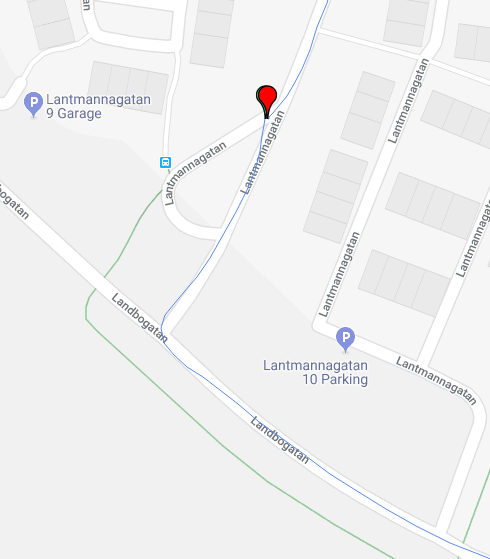
\includegraphics[width=0.6\textwidth]{figures/stopped_before_end}
    \caption{Real-world example of a bus driver stopping roughly 45 meters before reaching the final bus stop.
    The red marker is the GPS position where the bus stopped and the bus icon on the map is the pre-determined position of the bus stop.
    The bus stops there for a few minutes before it drives off to the first bus stop for a new journey.
    The bus detection algorithm systematically does not identify these cases.}
    \label{fig:stopped-before-end}
\end{figure}

\subsection{Imprecise Algorithms: Final Bus Stop Missed}
This scenario occurs due to a mix of imprecision in the bus stop detection algorithm and human error.
The scenario is illustrated in Figure \ref{fig:stopped-before-end}.
The bus driver completes the journey of a particular bus line and reaches the final bus stop.
However, the "Internal Analysis" component does not detect that the bus stop has been reached.
This is due to the bus driver stopping the bus slightly roughly 45 meters before the final bus stop.
The bus stops there for a few minutes, before it drives to the first bus stop for the new bus line number which was assigned.

This systematically occurs at certain bus stops, due to there being a "waiting" space commonly used by bus drivers while waiting for a new journey to be assigned.
The scenario highlights a problem with the implemented bus stop detection algorithm.
The bus stop detection algorithm can be improved to both handle these scenarios and yield more precise bus stop detection.
An improved bus stop detection algorithm is proposed in Section \ref{sec:improving-bus-stop-detection}.

\subsection{Bus Stops}
Using the finite-state machine provides context to the \textit{ObservedPositionEvent} types.
The states introduced yield a simple way to visualise contextual paths, e.g. actual journeys for a particular bus line or the path a bus drives to start a journey under a new bus line number.
However, the context-providing finite-state machine solution does not handle events about a bus arriving, departing or passing a bus stop on the journey.
Handling this type of data could be a critical step in detecting imprecisions in the bus stop detection algorithm or early stopping due to human error.
The "Started" state in the finite-state machine can easily be extended to not only include \textit{ObservedPositionEvent} types, but also \textit{ArrivedEvent}, \textit{DepartedEvent}, and \textit{PassedEvent} types.
For example, a missed final bus stop could be identified by looking at all the bus stops added to the "Started" state for that journey and compare them to the bus stops in other journeys for that particular bus line.

\subsection{Results}
The results of the pre-processing step is a collection of journeys for each bus line.
A journey consists of all the \textit{ObservedPositionEvent}s sent by the bus while the finite-state machine was in the "Started" state and all the bus stops the bus arrived at, departed from or passed by.
Erroneous event type ordering was solved by sorting the events based on \textit{Event ID} and retroactively adding \textit{ObservedPositionEvent} in the "Assigned" state to the "Started" state in the case of early journey assignment.
Journeys with early stopping or missed final bus stops are still prevalent in the collection of journeys.
These can be detected by analysing the bus stops registered during a journey.
In this thesis, the faulty journeys will only be marked as anomalies and discarded.
An index-tree is constructed to quickly access all journeys for a bus with a particular \textit{Vehicle ID}.
A number of high-level problems can now be formulated by using the two results from the pre-processing steps.

\subsection{Discussion}
The faulty journeys are only marked as anomalies and discarded in this thesis.
The fraction of faulty journeys can be calculated and used as a baseline when comparing an improved bus stop detection algorithm with the existing one.
Faulty journeys can be categorised based on the error in the journey, e.g. a missed starting bus stop is a different error compared with a missed final bus stop.
The categorisation of faults could provide deeper insights into the dataset.
For example, the insights could be used to improve the bus stop detection algorithm or identify journeys where a particular error occurs regularly.    



